\chapter{Design}
\label{chapter:Design}
This chapter summarizes the design of the conformance and correspondence recovery system developed for this thesis and its integration in the \gls{MegaL/Xtext} environment.

\section{Recovery System Design}
This section summarizes the design of the conformance and correspondence recovery system developed for this thesis.

\subsection{Recovery Process}
The recovery process is a straight forward analysis of two artifacts.
Figure \ref{figure:RecovryProcess} shows a flowchart depicting this.
\begin{figure}[h!]
\begin{center}
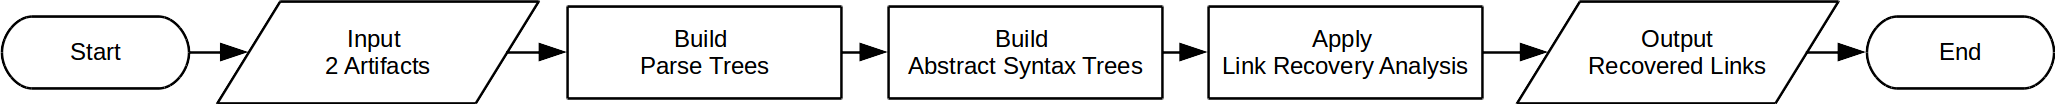
\includegraphics[width=\textwidth]{images/RecoveryProcess.png}
\end{center}
\caption{The Recovery Process}
\label{figure:RecovryProcess}
\end{figure}
Given two artifacts as input, the recovery process works as follows:
\begin{enumerate}
\item
From each artifact a \gls{CST} or \gls{ParseTree} is constructed,
\item
each \gls{ParseTree} is further refined into an \gls{AST},
\item
both \glspl{AST} are compared with each other, i.e. both trees are traversed in a \gls{DFS} fashion and each pair of nodes is checked whether it can be recovered as link.
\end{enumerate}
Eventually, the set of recovered links serves as output of the process.

\subsection{Recovery API}
The Recovery \gls{API} is the core of the developed recovery system.
It provides generalized data structures and methods for syntactic analysis of artifacts and their fragments.
Figure \ref{figure:RecoverySystemAPI} depicts the \gls{API} as block diagram.
\begin{figure}[h!]
\begin{center}
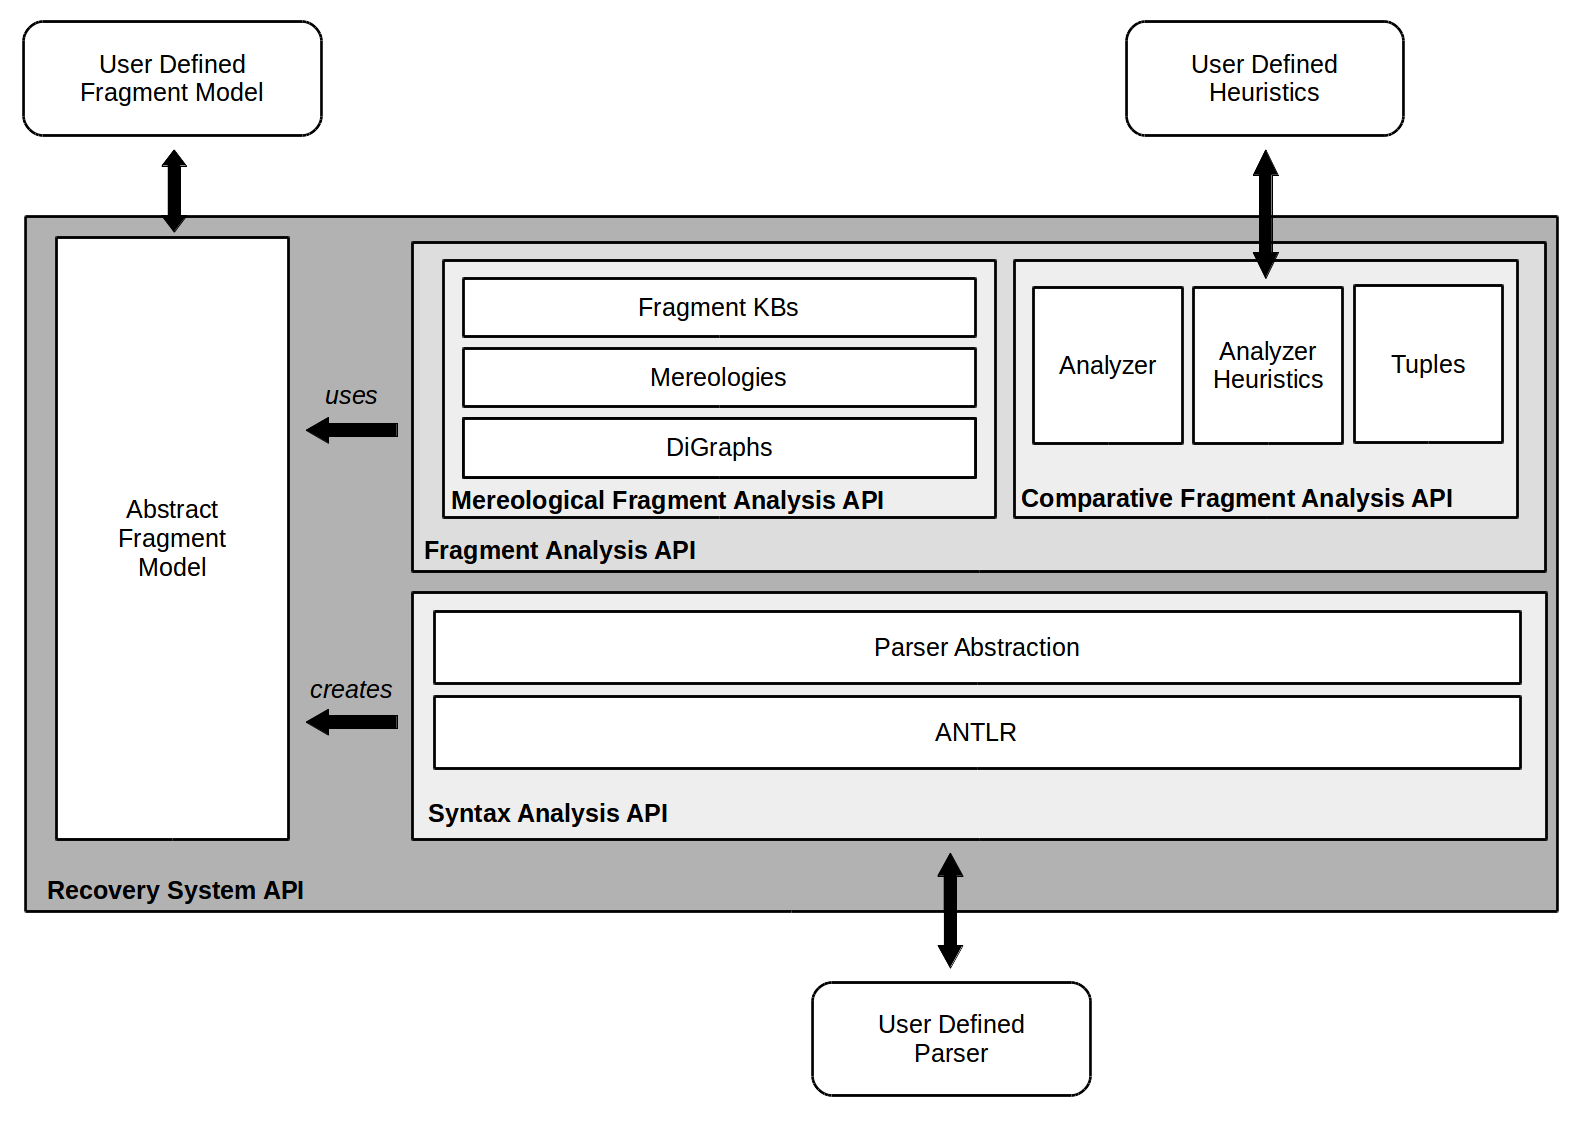
\includegraphics[width=\textwidth]{images/RecoverySystemAPI.png}
\end{center}
{
\scriptsize
This block diagram depicts the functional outline of the Recovery System \gls{API} (note, that this does not necessarily correspond to the package outline of its actual implementation).
}
\caption{The Recovery API}
\label{figure:RecoverySystemAPI}
\end{figure}
The components of the \gls{API} are:
\begin{description}

\item[Abstract Fragment Model]
The Abstract Fragment Model serves as base model for all \glspl{AST}.
It can thought of as \gls{DTO} for the analysis components.
As user of the \gls{API}, i have to derive a specific \gls{AST} from this model.
A detailed description follows in §\ref{subsubsection:AbstractFragmentModel}.

\item[Syntax Analysis API]
The Syntax Analysis \gls{API} is the abstraction layer for parsing and \gls{AST} construction.
It is currently backed by \gls{ANTLR}, but its internal design is loosely coupled, so other parser libraries can be used.
As user of the \gls{API}, i have to implement a parser constructing an \gls{AST} deriving the Abstract Fragment Model.
However, if one uses \gls{ANTLR}, only \gls{AST} construction from a \gls{CST} is required.
A detailed description follows in §\ref{subsubsection:SyntaxAnalysisAPI}.

\item[Fragment Analysis API]
The Fragment Analysis \gls{API} consists of two components:
\begin{description}

\item[Mereological Fragment Analysis API]
The Mereological Fragment Analysis \gls{API} provides components for deriving parthood links between syntactically well-formed fragments.
As user of the \gls{API}, i only have to apply its components to constructed \glspl{AST}.
A detailed description follows in §\ref{subsubsection:MereologicalFragmentAnalysisAPI}.

\item[Comparative Fragment Analysis API]
The Comparative Fragment Analysis \gls{API} provides components for deriving links between different artifacts and their fragments.
As user of the \gls{API}, i have to implement one or more specialized heuristics for deciding which links can be recovered.
A detailed description follows in §\ref{subsubsection:ComparativeFragmentAnalysisAPI}.

\end{description}

\end{description}

\subsubsection{Abstract Fragment Model}
\label{subsubsection:AbstractFragmentModel}
The Abstract Fragment Model describes a tree in which each node represents an syntactically well-formed fragment.
Figure \ref{figure:FragmentModel} shows an \gls{UML} class diagram of the model.
\begin{figure}[h!]
\begin{center}
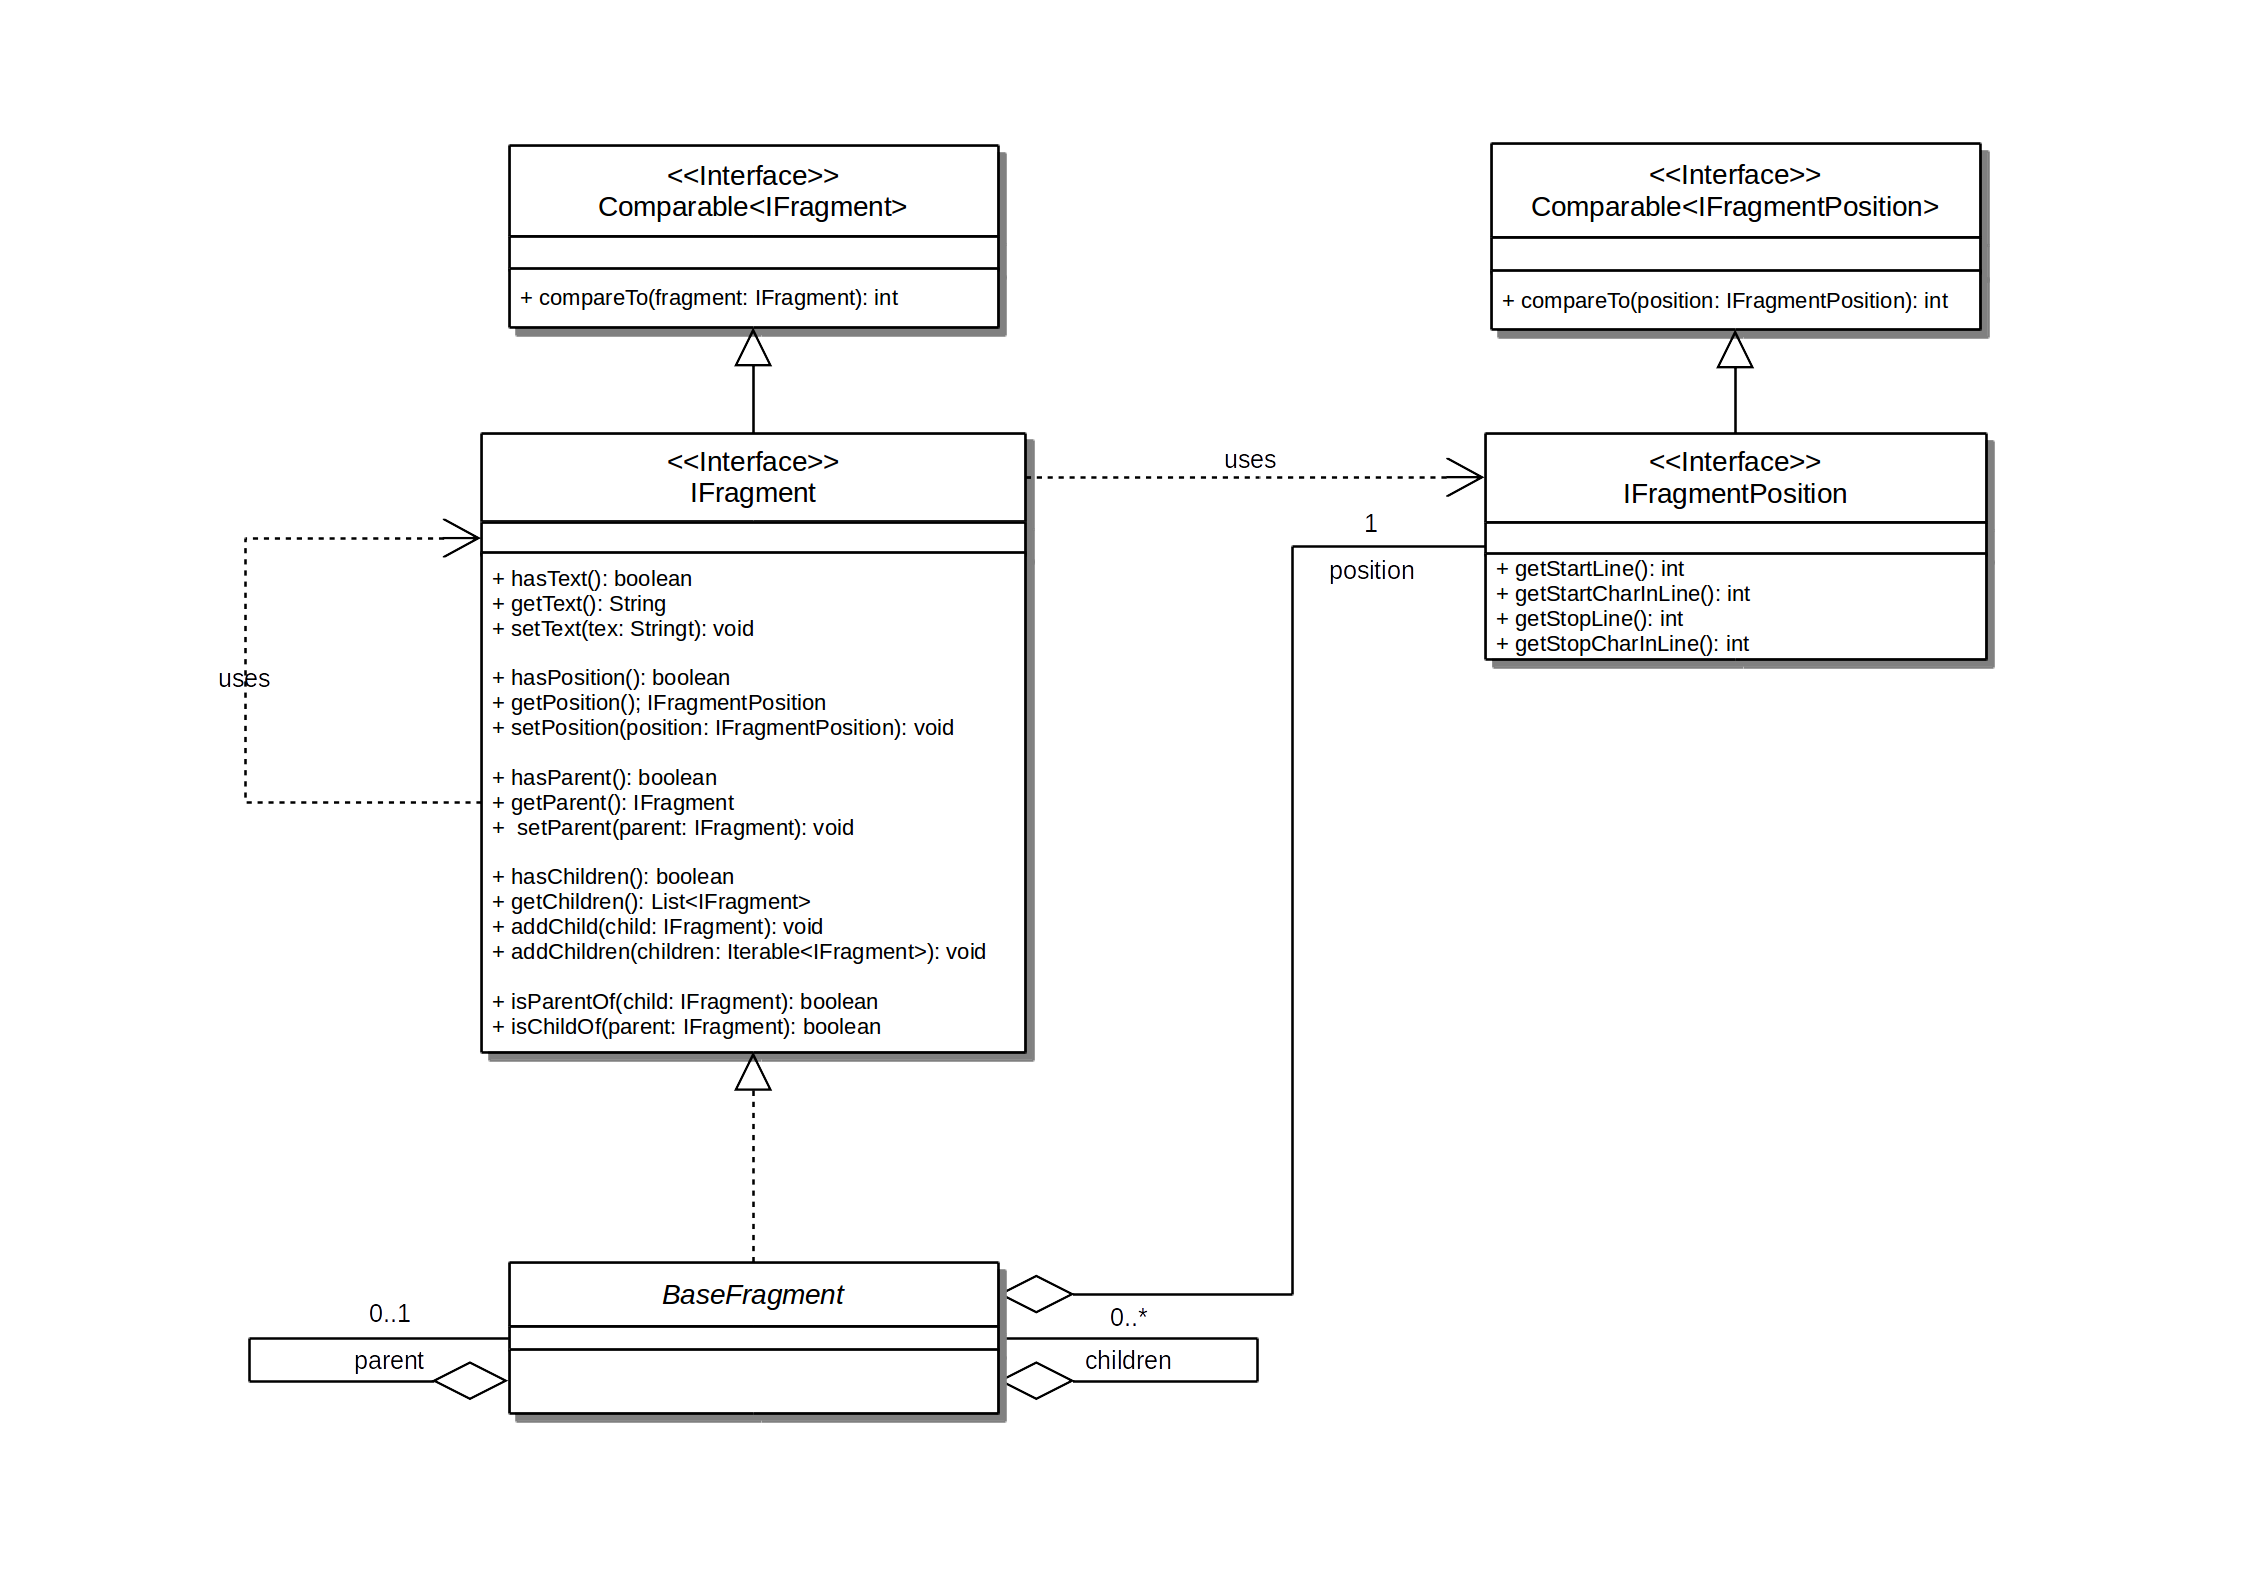
\includegraphics[width=\textwidth]{images/FragmentModel.png}
\end{center}
\caption{The Abstract Fragment Model}
\label{figure:FragmentModel}
\end{figure}
The resulting tree data structure is doubly-linked, i.e. an \texttt{IFragment} node aggregates references to its children an to its parent, given it is not the root node.
Each fragment \texttt{IFragment} contains the text it represents.
In order to distinguish fragments which represent the same text, each node also carries the text's position in the artifact through \texttt{IFragmentPosition} instances.
Positions inside the text are determined by the start and ending line number as well as the corresponding first and last character inside the line.
Most of \texttt{IFragment}'s relevant code for trees is pre-implemented in the \texttt{BaseFragment} abstract class.

\subsubsection{Syntax Analysis API}
\label{subsubsection:SyntaxAnalysisAPI}
The Syntax Analysis \gls{API} provides abstraction for \gls{AST} construction.
The \gls{API} itself is really small, it only consists of the \texttt{IParser} and \texttt{IParserFactory} interfaces.
However, its implementation for \gls{ANTLR} is designed to reduce \gls{ANTLR}-specific boilerplate code.
Figure \ref{figure:SyntaxAnalysisAPI} shows the \gls{UML} class diagram for the \gls{ANTLR} backed implementation.
\begin{figure}[h!]
\begin{center}
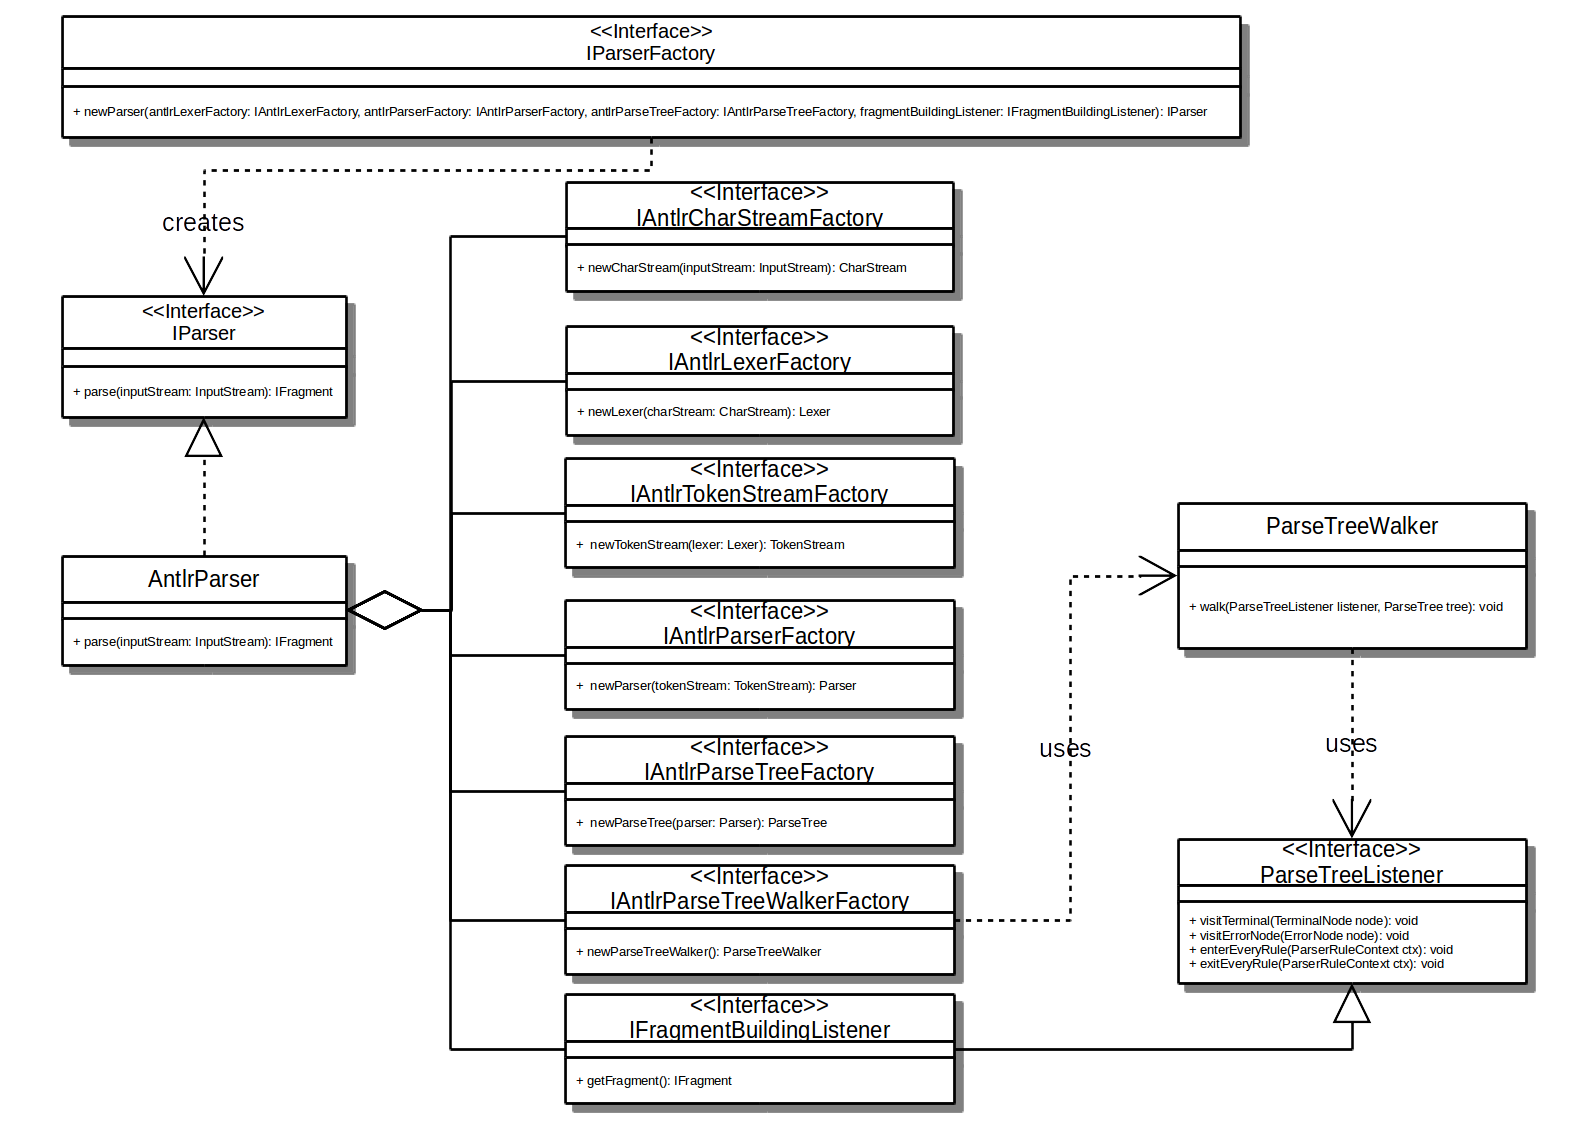
\includegraphics[width=\textwidth]{images/SyntaxAnalysisAPI.png}
\end{center}
\caption{The Syntax Analysis API}
\label{figure:SyntaxAnalysisAPI}
\end{figure}
One can see, that this implementation makes heavy use of the \gls{AbstractFactoryPattern}.
This allows for a quick and easy definition of new parsers as shown in Figure \ref{figure:IParserFactoryUsageExample}.

\begin{figure}[h!]
\begin{lstlisting}[language=Java]
...
IParser java8Parser = parserFactory.newParser(
	Java8Lexer::new,
	Java8Parser::new, 
	Java8Parser::compilationUnit, 
	Java8FragmentBuildingListener::new);
...
\end{lstlisting}
{
\scriptsize
This example demonstrates the creation of a new parser using an \texttt{IParserFactory} instance with \gls{Java}8 features.
Lexer and Parser classes are generated by \gls{ANTLR}.
A suitable listener has to be implemented.
}
\caption{\texttt{IParserFactory} Usage Example}
\label{figure:IParserFactoryUsageExample}
\end{figure}

The other advantage of the \gls{AbstractFactoryPattern} is that the instantiation of all relevant classes necessary for the creation of \gls{ANTLR} \glspl{ParseTree} takes place in the predefined \texttt{AntlrParser} class.
This is exemplified by Figure \ref{figure:AntlrParserParseTreeCreation}.

\begin{figure}[h!]
\begin{lstlisting}[language=Java]
...
CharStream charStream = antlrCharStreamFactory.newCharStream(inputStream);
Lexer lexer = antlrLexerFactory.newLexer(charStream);
TokenStream tokenStream = antlrTokenStreamFactory.newTokenStream(lexer);
Parser parser = antlrParserFactory.newParser(tokenStream);
ParseTree parseTree = antlrParseTreeFactory.newParseTree(parser);
...
\end{lstlisting}
{
\scriptsize
This example demonstrates the creation of an \gls{ANTLR} \texttt{ParseTree} instance as implemented by the \texttt{AntlrParser} class.
}
\caption{\texttt{AntlrParser} \gls{ParseTree} Creation}
\label{figure:AntlrParserParseTreeCreation}
\end{figure}

Creation of \glspl{AST} or fragment trees is done using the \texttt{ParseTreeWalker} and \texttt{ParseTreeListener} infrastructure provided by \gls{ANTLR} \cite{Parr:2013:DAR:2501720}.
This is an variation of the \gls{ObserverPattern}.
Listeners in conjunction with walkers are an alternative to the \gls{VisitorPattern} provided by \gls{ANTLR}.
An instance of \texttt{Parse\-Tree\-Walker} traverses a \gls{ParseTree} using \gls{DFS}.
During traversal, a designated method of \texttt{Parse\-Tree\-Listener} is executed.
For \gls{AST} creation, an \gls{API} user has to implement the \texttt{IFragmentBuildingListener} interface, which is an extension of the \texttt{ParseTreeListener} interface.
The creation of a fragment tree by \texttt{AntlrParser} is exemplified in Figure \ref{figure:AntlrParserFragmentCreation}.

\begin{figure}[h!]
\begin{lstlisting}[language=Java]
...
ParseTreeWalker parseTreeWalker = antlrParseTreeWalkerFactory.newParseTreeWalker();
parseTreeWalker.walk(fragmentBuildingListener, parseTree);
IFragment fragment = fragmentBuildingListener.getFragment();
...
\end{lstlisting}
{
\scriptsize
This example demonstrates the creation of an \texttt{IFragment} \gls{AST} instance as implemented by the \texttt{AntlrParser} class.
}
\caption{\texttt{AntlrParser} Fragment Creation}
\label{figure:AntlrParserFragmentCreation}
\end{figure}

\subsubsection{Mereological Fragment Analysis API}
\label{subsubsection:MereologicalFragmentAnalysisAPI}
The Mereological Fragment Analysis \gls{API} provides components for deriving \gls{Parthood} links between syntactically well-formed fragments.
Direct \gls{Parthood} links are recovered from parent/child relationships within an \texttt{IFragment} \gls{AST}.
However, because \gls{Parthood} is transitive, we also need to recover these links.
This is done using a digraph data structure upon which we can compute its reflexive transitive closure.

Figure \ref{figure:MereologicalFragmentAnalysisAPI} shows an \gls{UML} class diagram depicting the relevant classes and interfaces of the Mereological Fragment Analysis \gls{API}.
\begin{figure}[h!]
\begin{center}
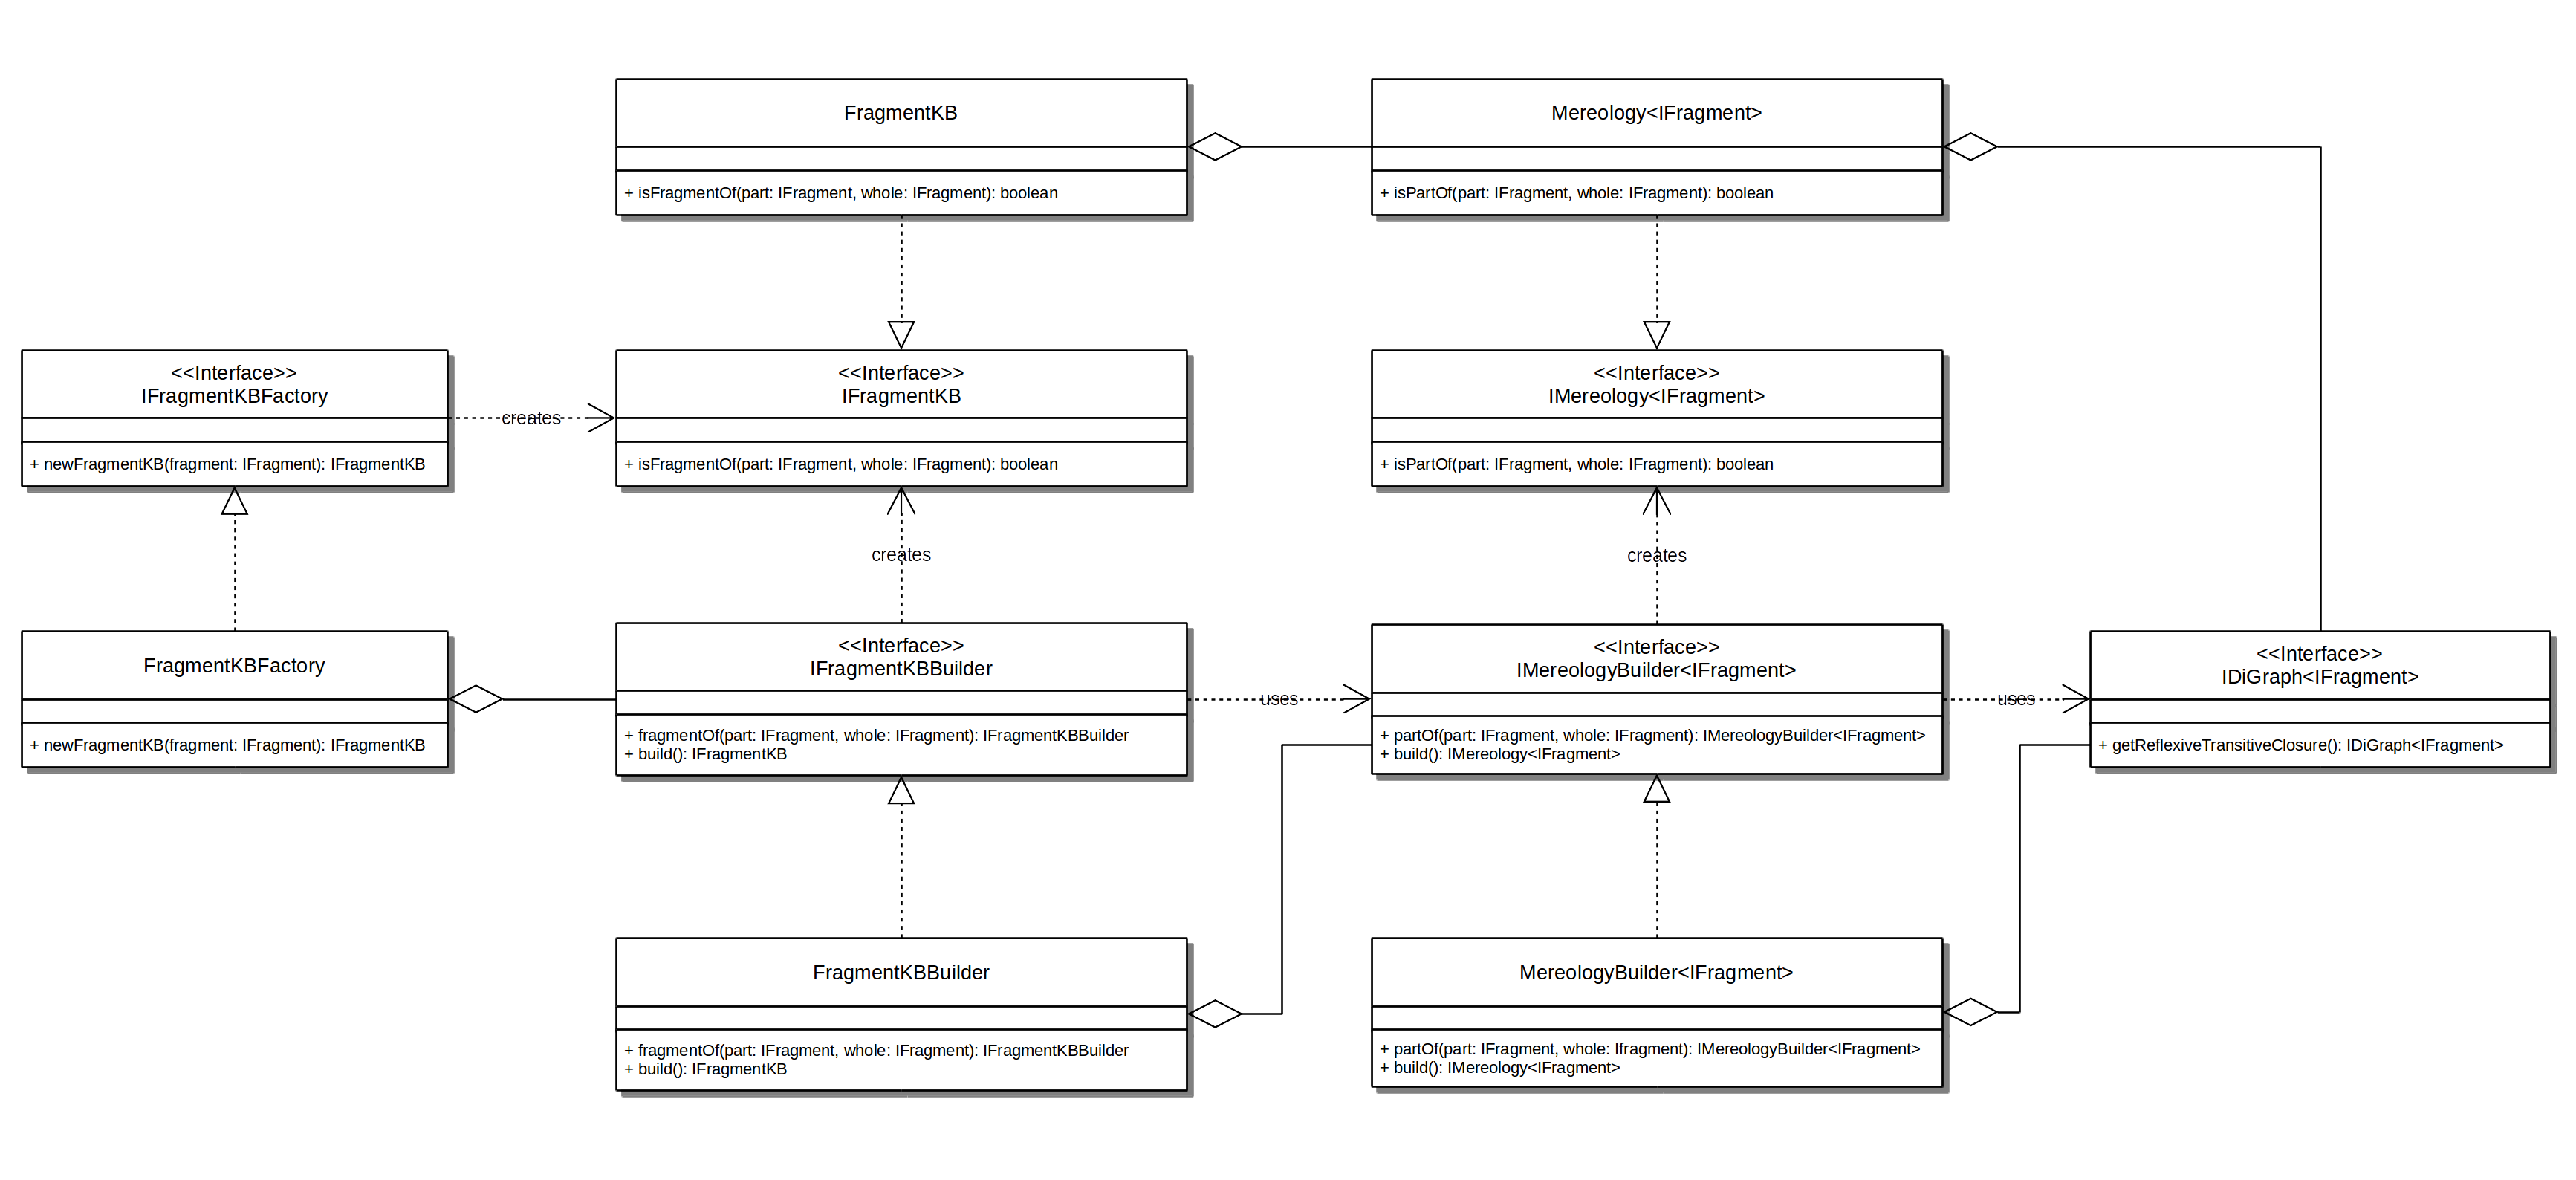
\includegraphics[width=\textwidth]{images/MereologicalFragmentAnalysisAPI.png}
\end{center}
\caption{Mereological Fragment Analysis API}
\label{figure:MereologicalFragmentAnalysisAPI}
\end{figure}
At its heart, the \gls{API} utilizes the generic \texttt{IDiGraph} interface whose implementations provide means for interrelating comparable objects, i.e. \texttt{IFragment} instances.

This digraph is wrapped by generic \texttt{IMereology} implementations, a data structure providing query methods on the topic of \gls{Mereology}, i.e. \gls{Parthood} relations.
\Glspl{Mereology} are constructed using the \gls{BuilderPattern}.
An \texttt{IMereology\-Builder} instance adds nodes and edges into its digraph with semantically named methods allowing a descriptive programming style.

\texttt{IMereology}'s are then further wrapped by \texttt{IFragmentKB} (a Knowledge Base over \texttt{IFragment}) implementations in order to avoid dealing with generics throughout the system.
This is also done utilizing the \gls{BuilderPattern}.

The recovery of \gls{Parthood} links is encapsulated through \texttt{IFragmentKB\-Factory} using the \gls{AbstractFactoryPattern}, which computes \texttt{IFragmentKB} instances from an \texttt{IFragment} \gls{AST} as input.


\subsubsection{Comparative Fragment Analysis API}
\label{subsubsection:ComparativeFragmentAnalysisAPI}
The Comparative Fragment Analysis \gls{API} provides components for deriving links from two \texttt{IFragment} \glspl{AST} generated from different artifacts.
\begin{figure}[h!]
\begin{center}
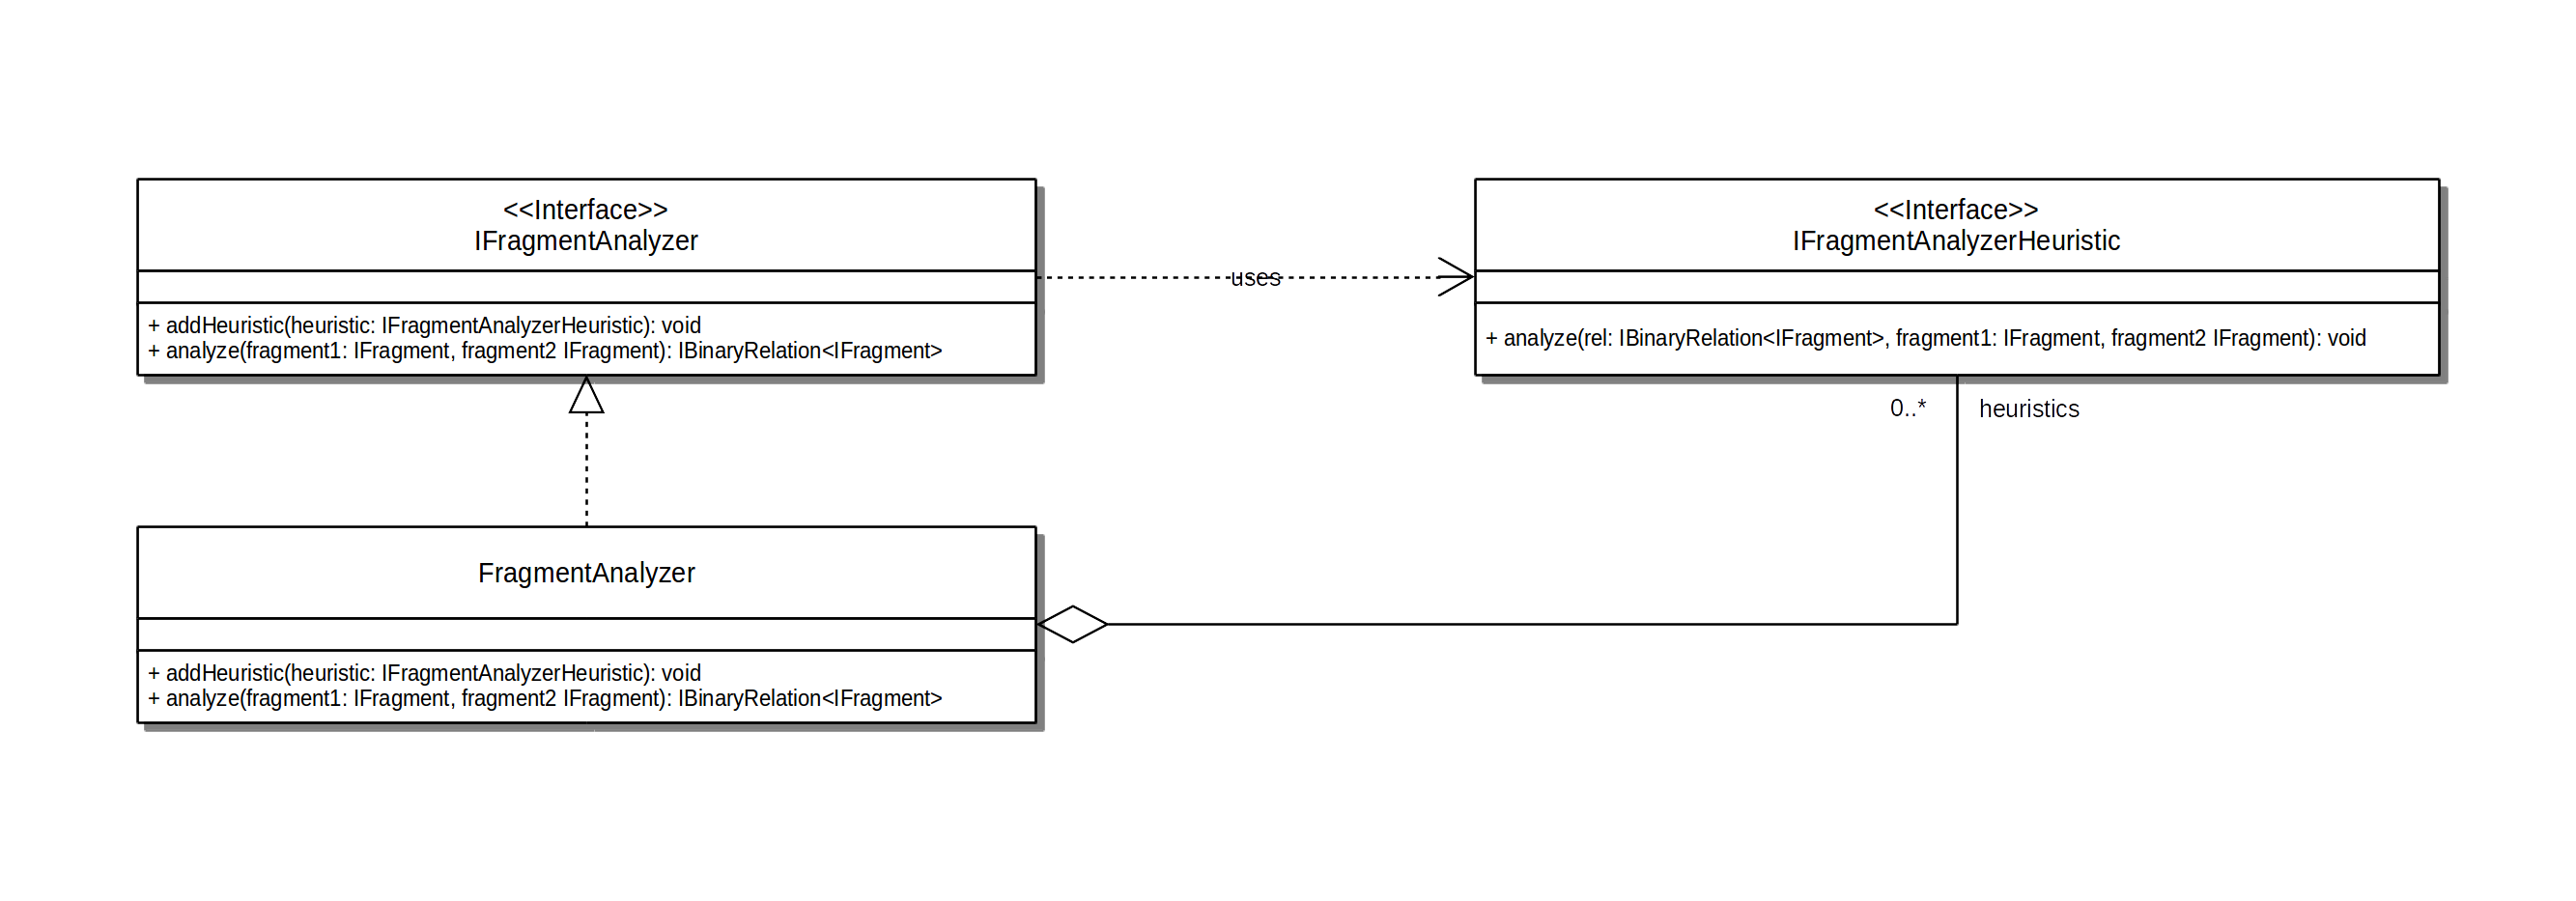
\includegraphics[width=\textwidth]{images/ComparativeFragmentAnalysisAPI.png}
\end{center}
\caption{Comparative Fragment Analysis API}
\label{figure:ComparativeFragmentAnalysisAPI}
\end{figure}
Figure \ref{figure:ComparativeFragmentAnalysisAPI} shows an \gls{UML} class diagram depicting the relevant interfaces and classes of the \gls{API}.
It utilizes the \gls{StrategyPattern} through the \texttt{IFragmentAnalyzerHeuristic} interface since concrete behavior of the recovery analysis is for the user to implement.
In this context, strategies are called heuristics, because recovery of links is not necessarily based on optimal, i.e. absolutely correct, solutions.
Instead strategies may also implement practical solutions with reasonably sufficient results.

\texttt{IFragmentAnalyzer} objects allow one to apply multiple heuristics, since there may be more than one practical approach to achieve a goal. Also this allows strategies to keep a relatively small implementation footprint.

Recovered links are captured and stored in an \texttt{IBinaryRelation} instance which works like a set of pairs.

\subsection{Recovery System}
\label{subsection:RecoverySystem}
The Recovery System is the actual implementation of \gls{Parthood}, \gls{Correspondence} and \gls{Conformance} link recovery for Java based \gls{O/R/X-Mapping} artifacts.
Figure \ref{figure:RecoverySystem} shows a block diagram outlining the functional components of the system.

\begin{figure}[h!]
\begin{center}
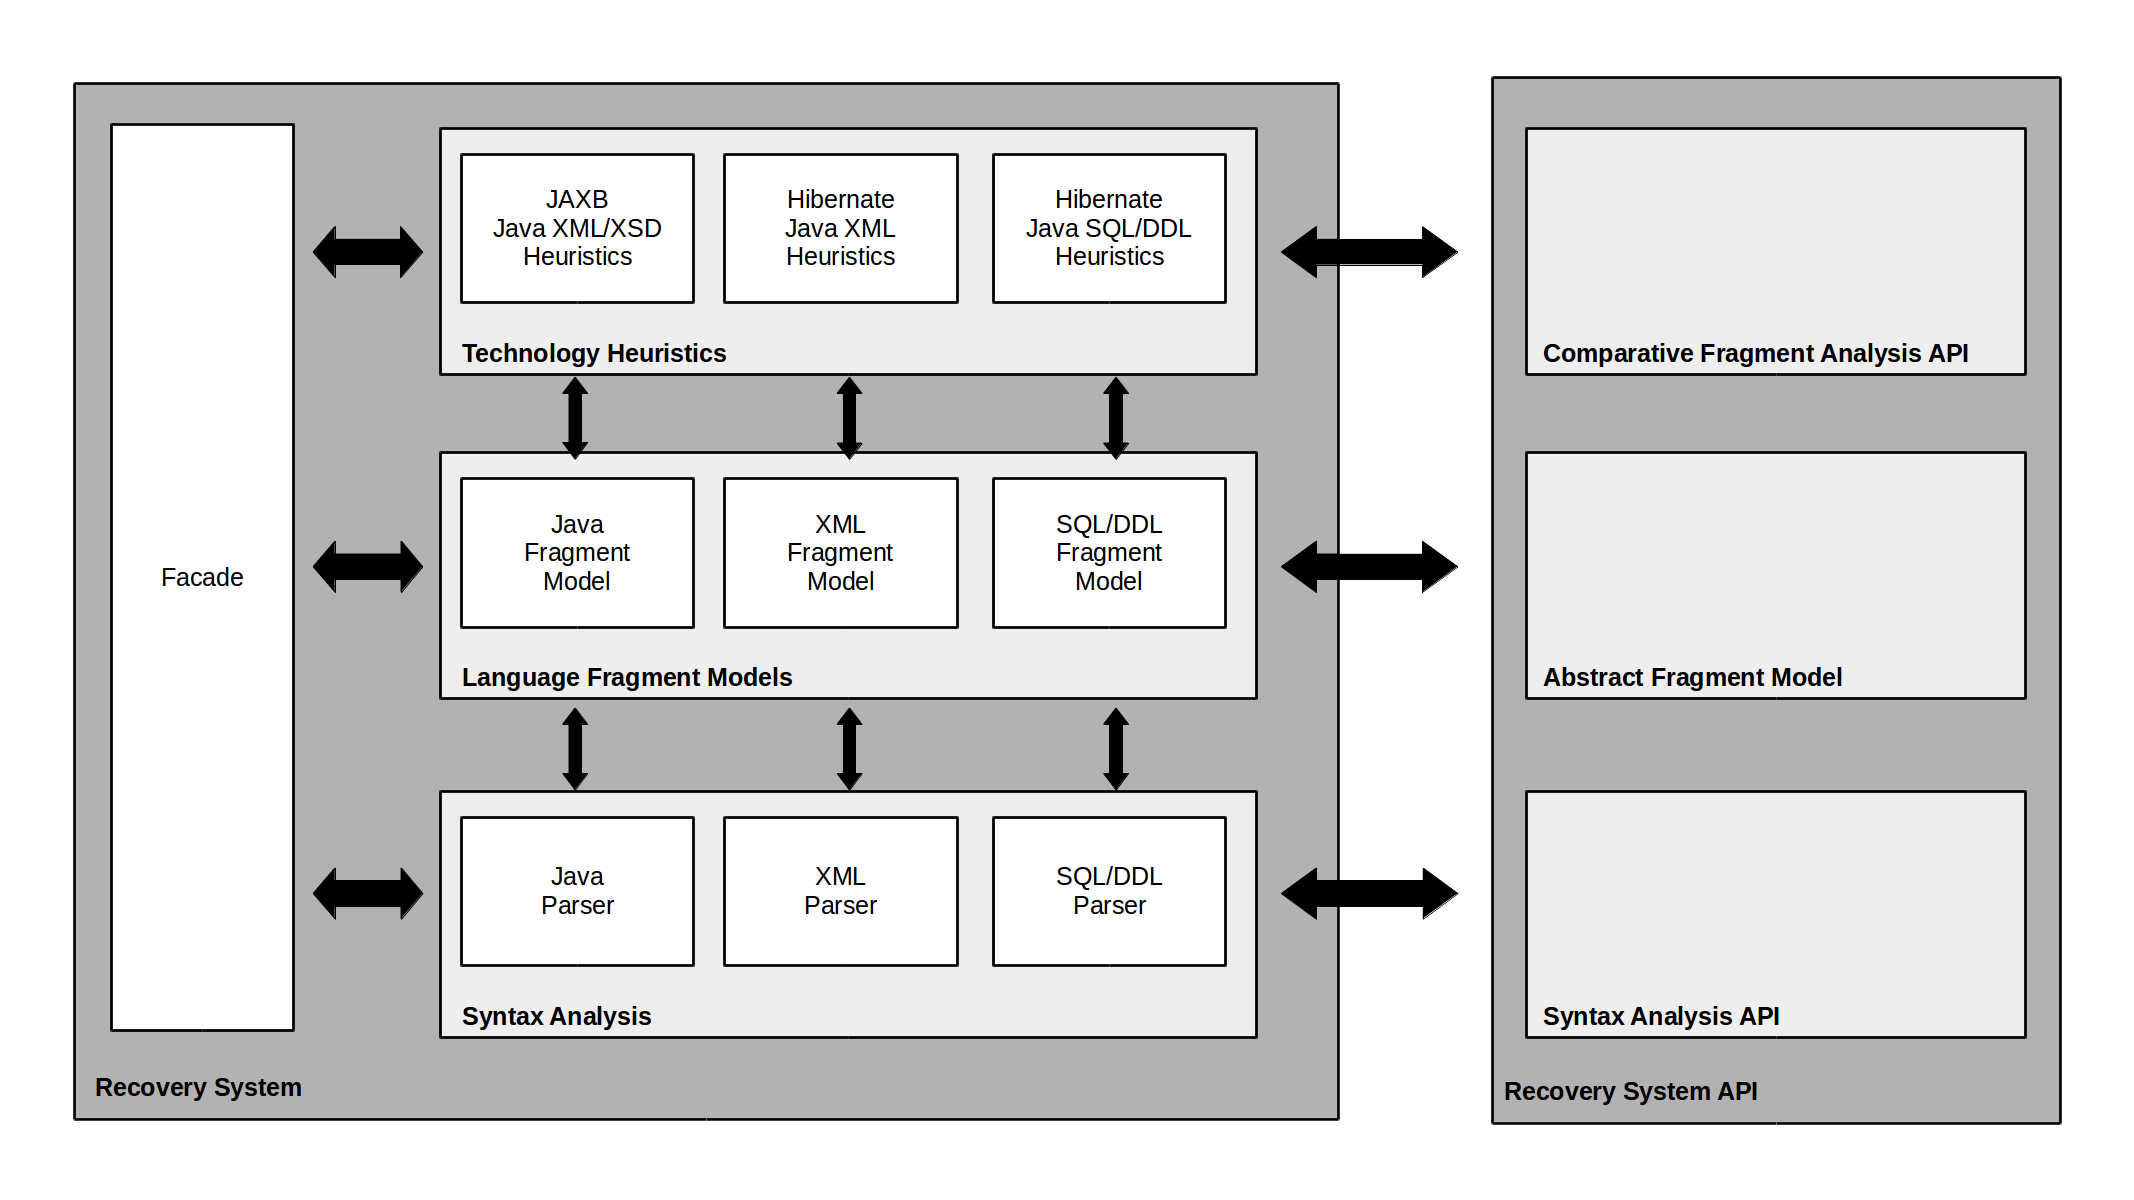
\includegraphics[width=\textwidth]{images/RecoverySystem.png}
\end{center}
{
\scriptsize
This block diagram depicts the functional outline of the Recovery System and its dependencies to the Recovery System \gls{API} (note, that this does not necessarily correspond to the package outline of its actual implementation).
}
\caption{The Recovery System}
\label{figure:RecoverySystem}
\end{figure}

The Recovery System utilizes the Syntactic Analysis \gls{API} described in §\ref{subsubsection:SyntaxAnalysisAPI} for \gls{Java}, \gls{XML} and \gls{SQL/DDL}.
For this, the Abstract Fragment Model described in §\ref{subsubsection:AbstractFragmentModel} is implemented.
Note, fragment models do not implement \gls{AST} suitable for compilation of the targeted language.
Syntactic features unnecessary for the intended analysis, like local variable declarations, arithmetic expressions or invocations, are omitted.
Fragment models rather focuses on structural features of the languages at hand.

The Comparative Fragment Analysis \gls{API} described in §\ref{subsubsection:ComparativeFragmentAnalysisAPI} is implemented with focus on artifacts of technologies, namely \gls{JAXB} and \gls{Hibernate}.
It implements heuristics for link recovery between:
\begin{itemize}
\item
\gls{Java} and \gls{XML} for \gls{JAXB} artifacts, i.e. \gls{Java} models are serialized as \gls{XML}
\item
\gls{Java} and \gls{XSD} for \gls{JAXB} artifacts, i.e. \gls{Java} models are serialized as \gls{XSD}
\item
\gls{XML} and \gls{XSD} for \gls{JAXB} artifacts, i.e. the two previous scenarios occurred
\item
\gls{Java} and \gls{XML} for \gls{Hibernate} mapping artifacts, i.e. \gls{Hibernate} uses \gls{XML} meta-data for \gls{O/R-Mapping}.
\item
\gls{Java} and \gls{SQL/DDL} for \gls{Hibernate} generated \gls{SQL} artifacts, i.e. \gls{Hibernate} uses \gls{Java} annotations for \gls{O/R-Mapping}
\end{itemize}

On top of the actual implementation, the Recovery System also utilizes the \gls{FacadePattern}.
This is to provide a single access point for all implemented analysis features.

\section{Megal/Xtext Integration Design}
This section summarizes the design of the recovery system's integration in the \gls{MegaL/Xtext} environment.
Figure \ref{figure:MegalXtextIntegrationDesign} shows a block diagram depicting the outline this integration.
Note, the Recovery System is implemented as separate project, which is then included as reference (through a \texttt{.jar} file) in a \gls{MegaL/Xtext} project.

\begin{figure}[h!]
\begin{center}
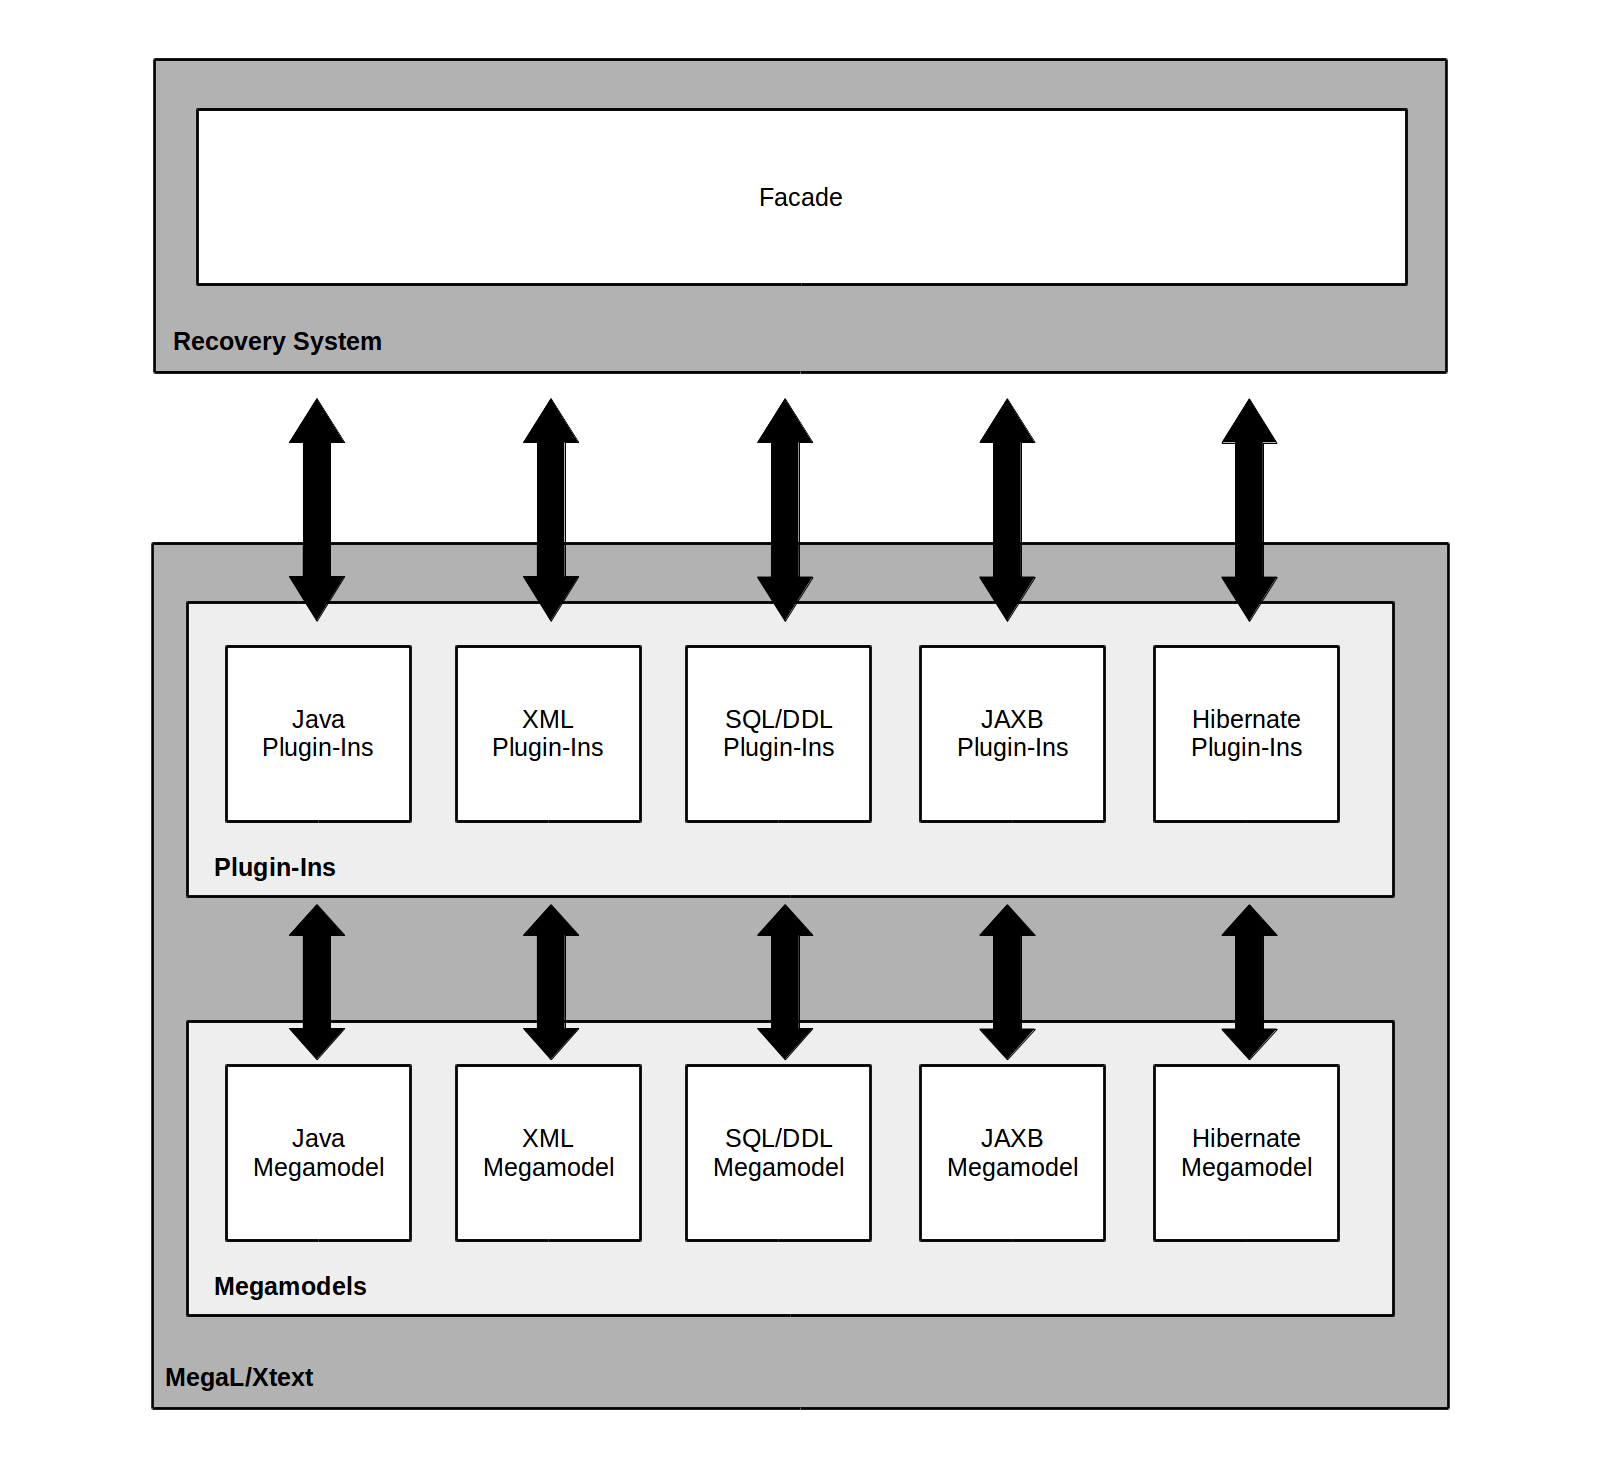
\includegraphics[width=\textwidth]{images/MegalXtextIntegrationDesign.png}
\end{center}
{
\scriptsize
This block diagram depicts the functional outline of the Recovery System's integration into the \gls{MegaL/Xtext} environment (note, that this does not necessarily correspond to the outline of its actual implementation).
}
\caption{Integration of the Recovery System int MegaL/Xtext}
\label{figure:MegalXtextIntegrationDesign}
\end{figure}

\gls{MegaL/Xtext} provides a plug-in system, which allows to bind special \gls{Java} classes to \texttt{Plugin} entities.
Code of such classes is then executed during the evaluation of a \gls{Megamodel}.
\ToDo{needs reference}
Figure \ref{figure:MegaLPluginInstantiation} exemplifies the declaration of Plug-in withing \gls{MegaL}.

\begin{figure}[h!]
\begin{lstlisting}
...
JavaFragmentRecoveryPlugin : Plugin
JavaFragmentRecoveryPlugin realizationOf Java
JavaFragmentRecoveryPlugin partOf FileFragmentRecoveryReasonerPlugin
JavaFragmentRecoveryPlugin = 'classpath:org.softlang.megal.plugins.impl.java.JavaFragmentRecoveryPlugin'
...
\end{lstlisting}
{
\scriptsize
This snippet demonstrates the instantiation of \texttt{JavaFragmentRecoveryPlugin} as part of \texttt{FileFragmentRecoveryReasonerPlugin} in \gls{MegaL}.
}
\caption{MegaL Plug-In Instantiation}
\label{figure:MegaLPluginInstantiation}
\end{figure}

The Recovery System or rather its facade (see §\ref{subsection:RecoverySystem}) is used to implement \gls{MegaL} plug-ins.
These Plug-ins are then in turn bound within \glspl{Megamodel}, which are divided by language and technology, i.e. there are separate \gls{MegaL} modules for \gls{Java}, \gls{XML}, \gls{SQL}, \gls{Hibernate} and \gls{JAXB}.
